% Aesthetic Computer --- Stack Knowledge (DevOps map poster)
% arxiv-style LaTeX poster. Build on neo or in the devcontainer (this Mac has no
% xelatex):  cd stack && latexmk -pdf stack-poster.tex   (or: pdflatex twice)
% Requires the `tikzposter` class (TeX Live full has it).
%
% Data assembled 2026-07-15 from the monorepo (package.json + lockfiles + ncu),
% infra config (lith/, session-server/, oven/, feed/, grab/, oven-edge/), and
% vendor/env-name mapping. Dollar costs are NOT in the repo except the one marked
% real; every other cost cell is "usage" or "needs input" --- do not invent them.
%
% Vendor "logos": represented as brand-coloured chips (self-contained so this
% builds anywhere). Dropping in real logo art / OS favicons is a follow-up pass ---
% put PNGs in stack/logos/ and swap the \chip macro for \includegraphics.

\documentclass[25pt, a1paper, landscape, margin=10mm, innermargin=12mm,
               blockverticalspace=10mm, colspace=12mm, subcolspace=6mm]{tikzposter}

\usepackage{booktabs}
\usepackage{array}
\usepackage{xcolor}
\usetikzlibrary{positioning, arrows.meta}  % tikzposter loads tikz; these libs aren't auto-loaded

\tikzposterlatexaffectionproofoff  % drop the "made with tikzposter" footer

% ---- palette ------------------------------------------------------------
\definecolor{acink}{HTML}{111417}
\definecolor{acpaper}{HTML}{F4F1EA}
\definecolor{acaccent}{HTML}{E4572E}
\definecolor{acblue}{HTML}{2E5EAA}
\definecolor{acgreen}{HTML}{2A9D8F}
\definecolor{acamber}{HTML}{E9B44C}
\definecolor{acred}{HTML}{C1121F}
\definecolor{acgray}{HTML}{6B7280}

% brand-ish chip colours
\definecolor{cDO}{HTML}{0080FF}
\definecolor{cCF}{HTML}{F38020}
\definecolor{cMongo}{HTML}{00684A}
\definecolor{cRedis}{HTML}{FF4438}
\definecolor{cGoogle}{HTML}{4285F4}
\definecolor{cStripe}{HTML}{635BFF}
\definecolor{cAuth0}{HTML}{EB5424}
\definecolor{cOpenAI}{HTML}{10A37F}
\definecolor{cAnthropic}{HTML}{D97757}
\definecolor{cEleven}{HTML}{111111}
\definecolor{cTezos}{HTML}{2C7DF7}

\newcommand{\chip}[2]{\colorbox{#1}{\textcolor{white}{\scriptsize\bfseries\,#2\,}}}
\newcommand{\real}[1]{\textcolor{acgreen}{\bfseries #1}}
\newcommand{\tbd}{\textcolor{acgray}{\itshape needs input}}
\newcommand{\usg}{\textcolor{acgray}{\itshape usage}}
\newcommand{\warn}[1]{\textcolor{acred}{\bfseries #1}}

% ---- theme --------------------------------------------------------------
\usetheme{Default}
\usecolorstyle{Denmark}
\colorlet{blocktitlebgcolor}{acink}
\colorlet{blocktitlefgcolor}{acpaper}
\colorlet{backgroundcolor}{acpaper}
\colorlet{framecolor}{acink}

\title{\textbf{Aesthetic Computer --- Stack Knowledge}}
\author{DevOps map: hosts, data, edge, deps, vendors \& costs}
\institute{assembled 2026-07-15 from the monorepo (knot: aesthetic.computer/core) \quad|\quad
           only the \real{green} cost is documented in-repo; the rest need owner input}
\date{}

\begin{document}
\maketitle[titletotopverticalspace=8mm]

\begin{columns}

% ======================= COLUMN 1 =======================
\column{0.34}

\block{Compute hosts}{
\scriptsize
\begin{tabular}{@{}p{3.9cm}p{2.2cm}p{5.9cm}p{3.6cm}@{}}
\toprule
\textbf{host} & \textbf{provider} & \textbf{role} & \textbf{deploy} \\
\midrule
\textbf{lith} \newline lith.aesthetic.computer \newline 209.38.133.33 &
\chip{cDO}{DO} \newline s-2vcpu-4gb, sfo3 &
Production web: Express 5 + Caddy monolith. All /api, runtime .mjs, KidLisp, notepat build, knot$\leftrightarrow$GitHub mirror &
fish lith/deploy.fish \newline systemd lith.service (MemMax 3G) \\
\addlinespace
\textbf{session-server} \newline session-server.aesthetic.computer \newline 157.245.134.225 &
\chip{cDO}{DO} \real{\$7/mo} \newline 1vcpu-1gb, nyc1 &
Chat + single shared realtime room (Geckos WS+UDP). Loads chat history on boot ($\sim$45s). Tiny 1GB box $\Rightarrow$ mem-sensitive &
fish session-server/deploy.fish \newline systemd, node 20.17 (fnm) \\
\addlinespace
\textbf{oven} \newline oven.aesthetic.computer &
\chip{cDO}{DO} \real{\$96/mo} \newline 8vcpu-16gb, sfo3 &
Tape$\rightarrow$MP4 (ffmpeg/Sharp); AC Native OS OTA builds; git pollers &
fish oven/deploy.fish \newline systemd oven.service \\
\addlinespace
\textbf{dp1-feed} (Go) &
same lith host &
DP-1 Feed API, Go + Postgres, 127.0.0.1:8787 &
systemd dp1-feed.service \\
\bottomrule
\end{tabular}
\vspace{2mm}

\textbf{\warn{Note:}} Jamsocket (per-piece spawned backends) is \warn{deprecated} --- realtime is now the single droplet. Code refs still linger in session-server.
}

\block{Data stores}{
\footnotesize
\begin{tabular}{@{}p{3.4cm}p{4.2cm}p{7.4cm}@{}}
\toprule
\textbf{store} & \textbf{where} & \textbf{holds} \\
\midrule
\chip{cMongo}{MongoDB} & Atlas (\ldots qencn\ldots) & users, handles, chat, moods, builds \\
\chip{cRedis}{Redis} & \chip{cDO}{DO} Managed, sfo3 & session / realtime state \\
Postgres & local to dp1-feed host & DP-1 feed (Go) \\
DO Spaces (S3) & \chip{cDO}{DO} & asset CDN: art, tapes, wand, amxd \\
\chip{cGoogle}{Firebase} & Google & auth, push messaging \\
CF KV / R2 / Queues & \chip{cCF}{Cloudflare} & feed KV, ac-os-images R2, write queue \\
\bottomrule
\end{tabular}
}

\block{Mac fleet \& hardware}{
\footnotesize
\begin{tabular}{@{}p{2.6cm}p{2.6cm}p{8.6cm}@{}}
\toprule
\textbf{box} & \textbf{os} & \textbf{role} \\
\midrule
neo & macOS & primary dev; builds menubar/electron; deskflow KVM server (8GB) \\
blueberry & macOS & Xcode 26.5 + Metal; Menu Band App Store builds \\
panda & macOS & Iris/Fuser tooling; deskflow client \\
chicken & macOS & fleet client (Ableton, menubar) \\
macbook-pro-clam & macOS (M1) & viewer; kidlispkids hourly art loop \\
jas-nzxt & \chip{acblue}{Fedora} & RTX 3070 BTX miner \\
jasellite & Linux (\chip{cDO}{DO}) & remote-claude box, 24.144.92.66 \\
\bottomrule
\end{tabular}
\vspace{1mm}
Meshed via toolchain/macos/fleet (ssh-mesh, stats-sync); tailnet network path.
}

% ======================= COLUMN 2 =======================
\column{0.32}

\block{Architecture}{
\centering
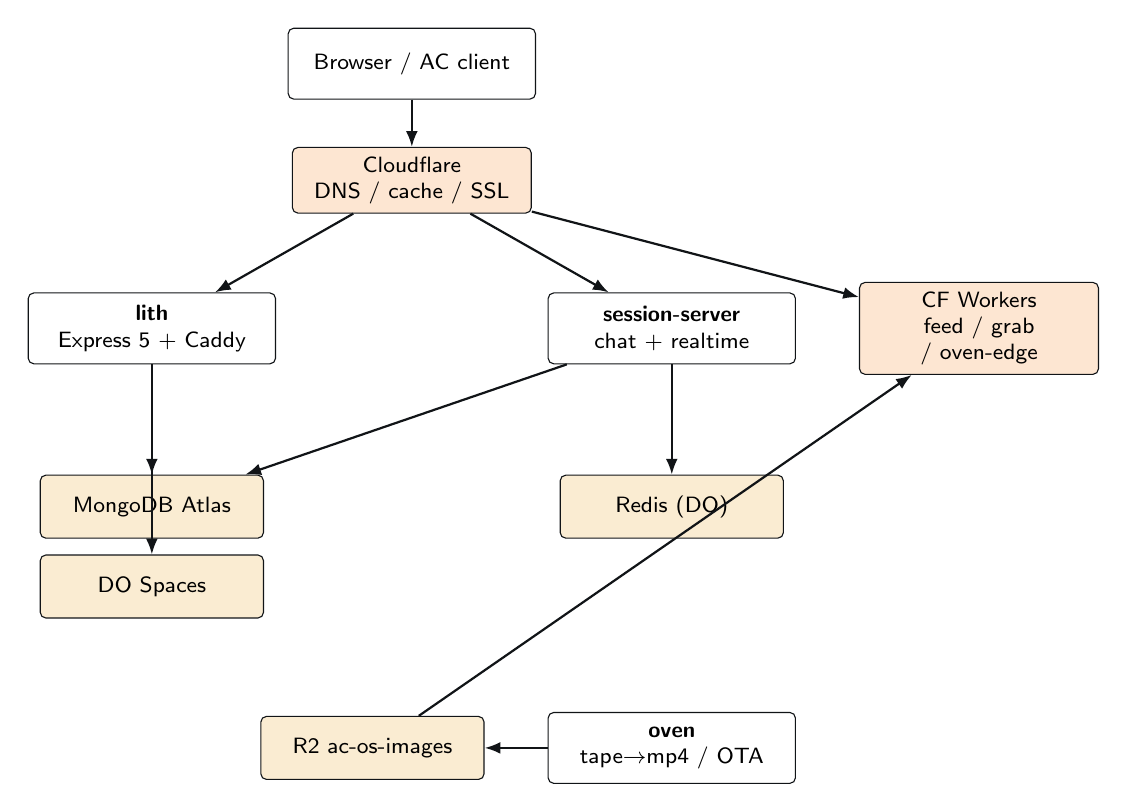
\begin{tikzpicture}[font=\footnotesize\sffamily, node distance=6mm,
  box/.style={draw=acink, rounded corners=2pt, fill=white, minimum height=9mm, text width=30mm, align=center, inner sep=2pt},
  store/.style={draw=acink, fill=acamber!25, rounded corners=2pt, minimum height=8mm, text width=26mm, align=center},
  edge/.style={draw=acink, fill=cCF!20, rounded corners=2pt, minimum height=8mm, text width=28mm, align=center},
  ar/.style={-{Latex[length=2mm]}, acink, thick}]

\node[box] (browser) {Browser / AC client};
\node[edge, below=of browser] (cf) {Cloudflare\\DNS / cache / SSL};
\node[box, below left=10mm and 2mm of cf] (lith) {\textbf{lith}\\Express 5 + Caddy};
\node[box, below right=10mm and 2mm of cf] (ss) {\textbf{session-server}\\chat + realtime};

\node[store, below=14mm of lith] (mongo) {MongoDB Atlas};
\node[store, below=2mm of mongo] (spaces) {DO Spaces};
\node[store, below=14mm of ss] (redis) {Redis (DO)};

\node[edge, right=8mm of ss] (workers) {CF Workers\\feed / grab / oven-edge};
\node[box, below=22mm of redis] (oven) {\textbf{oven}\\tape$\rightarrow$mp4 / OTA};
\node[store, left=8mm of oven] (r2) {R2 ac-os-images};

\draw[ar] (browser) -- (cf);
\draw[ar] (cf) -- (lith);
\draw[ar] (cf) -- (ss);
\draw[ar] (cf) -- (workers);
\draw[ar] (lith) -- (mongo);
\draw[ar] (lith) -- (spaces);
\draw[ar] (ss) -- (redis);
\draw[ar] (ss) -- (mongo);
\draw[ar] (oven) -- (r2);
\draw[ar] (r2) -- (workers);
\end{tikzpicture}
\vspace{1mm}

\scriptsize \textbf{git:} knot (git@knot.aesthetic.computer/core, what lith pulls) $\leftrightarrow$ GitHub mirror (whistlegraph/aesthetic-computer), synced every 60s by ac-mirror.timer on lith.
}

\block{Projects \& runtimes}{
\footnotesize
\begin{tabular}{@{}p{3.2cm}p{3.0cm}p{7.6cm}@{}}
\toprule
\textbf{project} & \textbf{runtime} & \textbf{deploys to} \\
\midrule
system & Node & lith (Express+Caddy) \\
session-server & Node 20 & DO droplet (systemd) \\
lith & Node ESM (express 5) & the monolith itself \\
oven & Node $\geq$20 (express 4) & oven droplet \\
dp1-feed & Cloudflare Worker + Go & wrangler / systemd \\
grab & CF Worker (Browser Rendering) & grab.aesthetic.computer \\
oven-edge & CF Worker + R2 & os.aesthetic.computer \\
ac-electron & Electron 39 & releases.aesthetic.computer \\
vscode-extension & VS Code ext & Marketplace (v1.274) \\
mcp-server & Node $\geq$18 & npm @aesthetic.computer/mcp \\
nanos & Node 20 unikernel & NanoVMs ops $\rightarrow$ GCP/DO \\
\bottomrule
\end{tabular}
\vspace{1mm}

\textbf{non-JS:} \chip{acaccent}{C} fedac/native (AC Native OS) \; \chip{acaccent}{Rust} ac-event-daemon, vello-wasm \; \chip{acaccent}{Swift} slab menubar (App Store) \; \chip{acaccent}{LaTeX} papers \; \chip{acaccent}{WASM} vello, fedac.
}

\block{Version skew \& risk}{
\footnotesize
\textbf{Skew across sub-projects:}\\
mongodb \textbf{6} (root/oven/nanos) vs \textbf{7} (system/session) \\
@aws-sdk 3.540 (oven) / 3.934 (root) / 3.1020 (system) \\
@taquito \textbf{24} (root) vs \textbf{25} (system) \quad express \textbf{4} (oven) vs \textbf{5} (lith) \\[1mm]
\textbf{Abandoned / EOL:} \warn{gpt3-tokenizer}, \warn{gotrue-js} (Netlify Identity, off-host), \warn{ntp-client} ($\sim$9y), Netlify CLI (legacy dev baggage). \\[1mm]
\textbf{Open:} two feed impls both target feed.aesthetic.computer (Go svc + CF Worker) --- one may be dead. dp1-feed submodule not checked out.
}

% ======================= COLUMN 3 =======================
\column{0.34}

\block{Outdated (system \& session-server)}{
\footnotesize
\textbf{system/ --- major bumps available}\\
\begin{tabular}{@{}p{4.6cm}p{3.0cm}p{3.0cm}@{}}
\toprule
\textbf{package} & \textbf{current} & \textbf{latest} \\
\midrule
redis & 5.10.0 & 6.1.0 \\
got & 14.6.4 & 15.1.0 \\
gotrue-js & 0.9.29 & 1.0.1 \\
nanoid & 5.1.6 & 6.0.0 \\
adm-zip & 0.5.16 & 0.6.0 \\
gcp-metadata & 7.0.1 & 8.1.3 \\
typescript (dev) & 5.9.3 & 7.0.2 \\
\midrule
\multicolumn{3}{@{}l}{\textit{minor:} aws-sdk 3.1020$\rightarrow$3.1087, openai 6.46$\rightarrow$6.47, three 0.182$\rightarrow$0.185}\\
\bottomrule
\end{tabular}
\vspace{2mm}

\textbf{session-server/ --- intentionally pinned}\\
\begin{tabular}{@{}p{3.6cm}p{2.6cm}p{4.4cm}@{}}
\toprule
\textbf{package} & \textbf{state} & \textbf{why} \\
\midrule
geoip-lite & held 1.4.10 & 2.x needs Node $\geq$24 \\
ws & held 8.21.0 & 8.21.1 too new (cooldown) \\
redis & \warn{reverted to 4.7} & 6.x broke prod (see plan) \\
mongodb & \warn{reverted to 6.20} & bundled w/ redis revert \\
\bottomrule
\end{tabular}
}

\block{Vendors \& costs}{
\scriptsize
\begin{tabular}{@{}p{5.0cm}p{4.4cm}p{3.2cm}@{}}
\toprule
\textbf{vendor / use} & \textbf{billing} & \textbf{cost} \\
\midrule
\chip{cDO}{DO} Droplet --- lith host & subscription & \real{\$24/mo} \\
\chip{cDO}{DO} Droplet --- session-server & subscription & \real{\$7/mo} \\
\chip{cDO}{DO} Droplet --- oven (8vcpu/16gb) & subscription & \real{\$96/mo} \\
\chip{cDO}{DO} Droplet --- jasellite & subscription & \real{\$96/mo} \\
\chip{cDO}{DO} Droplets --- at, silo, help & subscription & \real{\$24 ea} \\
\chip{cDO}{DO} Droplet --- \warn{legacy-2016} & subscription & \real{\$12/mo} \\
\chip{cDO}{DO} Spaces --- asset CDN (11 keys) & storage + egress & on invoice \\
\chip{cRedis}{Valkey 8} --- DO managed, sfo3 & subscription & \real{$\sim$\$15/mo} \\
\multicolumn{3}{@{}p{12cm}}{\real{\textbf{DO total $\approx$\$330/mo}} and \warn{climbing} --- invoices Mar \$189 $\rightarrow$ Jun \$259.54; Jul \$172 by the 15th} \\
\midrule
\chip{cMongo}{MongoDB} Atlas --- primary DB & subscription/usage & \tbd \\
\chip{cCF}{Cloudflare} --- DNS/cache & free tier likely & \usg \\
\chip{cCF}{Cloudflare} --- Workers/KV/R2/Queues & usage & \usg \\
\chip{cCF}{Cloudflare} --- Browser Rendering (grab) & paid tier & \tbd \\
\chip{cGoogle}{Firebase} --- auth/push & free tier likely & \usg \\
\chip{cAuth0}{Auth0} --- identity (2 tenants) & free/paid tier & \tbd \\
\chip{cStripe}{Stripe} --- payments & per-txn \% & \usg \\
\chip{cGoogle}{Google Cloud} --- TTS + VMs & usage & \tbd \\
\chip{cOpenAI}{OpenAI} --- TTS/gen & per-token & \usg \\
\chip{cAnthropic}{Anthropic} --- agents & per-token & \usg \\
\chip{cEleven}{ElevenLabs} --- voice (PVC) & subscription/usage & \tbd \\
Buzzsprout --- podcast host & subscription & \tbd \\
\chip{cTezos}{Tezos}+Pinata --- minting/IPFS & gas + pinning & \usg \\
Printful --- merch fulfillment & per-order & \usg \\
Porkbun --- domains & per-domain/yr & \tbd \\
Netlify --- former host & \real{\$0 while idle} & \real{\$0} \\
\bottomrule
\end{tabular}
\vspace{1mm}

\scriptsize Also wired (names only): PayPal, SMTP, Browserless, NVIDIA API, Datomic (kidlisp), VAPID web-push (self-hosted, \$0), AT Proto/PDS (self-host).
}

\block{How to use this}{
\footnotesize
Build: \texttt{cd stack \&\& latexmk -pdf stack-poster.tex} on \textbf{neo} or the devcontainer.
Data spine lives in \texttt{stack/}. Cost cells marked \tbd{} need a billing snapshot; \usg{} = usage-metered (varies).
Real logos / OS favicons: drop PNGs in \texttt{stack/logos/} and swap the \texttt{\textbackslash chip} macro.
}

\end{columns}
\end{document}
